\documentclass[a4paper,twoside, 12pt]{memoir} %A4papir, to side, størrelse 12, type memoir 	
% For dansk opsætning med æ, ø og å, samt pænere orddeling.
\usepackage[utf8]{inputenc}	

%%%%%%%%%%%%%%%%%%%%%%%Opsætning af format%%%%%%%%%%%%%%%%%%%%%%%%%%
%\documentclass[a4paper,oneside]{memoir} %A4papir, en side, størrelse 12, type memoir 		

%\usepackage[danish,english]{babel}				% dansk og engelsk opsætning
\usepackage[english]{babel}				% dansk og engelsk opsætning
%\renewcommand{\danishhyphenmins}{22}			% fikser babel fejl/bedre orddeling
\usepackage[T1]{fontenc}
\usepackage{lmodern} 
\usepackage{csquotes}


%%Høre til under tabel (Pakker, men skal stå før pgfplot pga. default værdier)%%
\usepackage[table]{xcolor}	

\usepackage{graphicx} 				% Haandtering af eksterne billeder (JPG, PNG, EPS, PDF)
\usepackage{soul}
\usepackage{multirow}               % Fletning af raekker og kolonner (\multicolumn og \multirow)
\usepackage{wrapfig}				%for figure der skal have tekst om sig
\usepackage{float}					% Muliggoer eksakt placering af floats, f.eks. \begin{figure}[H]
\usepackage{enumerate}				% Muliggoer at man kan bruge fx a) i enumerate
\usepackage{pdflscape}				% Muligør landskab på enkelte sider
\usepackage{tabularx}				% Tabeller med X width
\usepackage{mathtools}				% Formler og matematik
\usepackage{pdfpages}				% til at inkludere PDF filer
\usepackage[footnote,draft,english,silent,nomargin]{fixme}	% For at holde styr på mangler i teksten
\usepackage{ifthen}					% If then
\usepackage{hyperref}
\usepackage{textcomp,gensymb}		% symboler til latex
\usepackage{enumitem}				% Muligheder for ref til item
\usepackage{amsfonts}

% ?? Using
%\usepackage[bottom]{footmisc} %fodnoter i bunden af arket

% Complains
% \usepackage{caption}

%--------------------------------------------------------------------
% Billeder bliver lagt i Media
%--------------------------------------------------------------------
\graphicspath{{../figs/}}

%--------------------------------------------------------------------
% Marginer
%--------------------------------------------------------------------
\usepackage{ragged2e,anyfontsize}							%Justering af elementer
\raggedbottom												%Ingen side strech for twopage
\setlrmarginsandblock{3cm}{3cm}{*}							%Højre - venstre
\setulmarginsandblock{3cm}{2.5cm}{*}						%Øverst - nederst
\checkandfixthelayout[nearest]    							%Specifikt valg af højde algoritme
% No more use 2015 \usepackage{fixltx2e}					%Retter forskellige fejl i LaTeX-kernen

%--------------------------------------------------------------------
%  Inholdsfortegnelse
%--------------------------------------------------------------------
\setcounter{tocdepth}{3} % inkludere sub + subsubsection i inholdsfortegnelde
\setsecnumdepth{subsection}


%--------------------------------------------------------------------
% Kapitel formatering
%--------------------------------------------------------------------
\usepackage{titlesec} 

%--------------------------------------------------------------------
% Sektion formatering
%--------------------------------------------------------------------
\titlespacing\section{0pt}
{24pt plus 4pt minus 2pt}{6pt plus 2pt minus 2pt} %halvt mellemrum efter section

\titlespacing\subsection{0pt}
{18pt plus 4pt minus 2pt}{2pt plus 2pt minus 2pt} %kun lidt mellemrum efter subsection

\titlespacing\subsubsection{0pt}
{18pt plus 4pt minus 2pt}{2pt plus 2pt minus 2pt} %kun lidt mellemrum efter subsubsection 

\setlength\parskip{0.2em plus 0.1em}
\setlength\parindent{15pt}



%--------------------------------------------------------------------
% Sidehoved og -fod
%--------------------------------------------------------------------
\let\footruleskip\undefined  %fixer memoir default footruleskip
\usepackage{fancyhdr}
\pagestyle{fancy}
\fancyhf{}
\fancyhead[C]{\textit{<title of thesis>}}
\fancyfoot[RO,LE]{\thepage\ of \thelastpage}  	% sættet sidetal tal h/v efter om der er ulige
												% eller lige sidetal

\fancypagestyle{plain}{% bruges ved Undtagelser						
  \fancyhf{}%
  \fancyfoot[RO,LE]{\thepage\ of \thelastpage}	
  \renewcommand{\headrulewidth}{0pt}			%Ingen linje ved chapter, kun sidetal
}

%--------------------------------------------------------------------
% Literaturliste liste
%--------------------------------------------------------------------
\usepackage{varioref}							% Muliggoer bl.a. krydshenvisninger med sidetal (\vref)
\usepackage{nameref}							% refference der udskriver navn
%\usepackage{natbib}							% Udvidelse med naturvidenskabelige citationsmodeller

%\bibpunct[,]{[}{]}{;}{a}{,}{,} 				% Definerer de 6 parametre ved Harvard henvisning 
												% (bl.a. parantestype og seperatortegn)
%\bibliographystyle{../Latex/Litteratur/plainnat}		% Udseende af litteraturlisten.
%\bibliographystyle{IEEEtranSN}
\usepackage[backend=bibtex,style=ieee,natbib=true,bibencoding=ascii,sorting=none]{biblatex}
\addbibresource{./literature.bib}
%--------------------------------------------------------------------
% Ordliste
%--------------------------------------------------------------------
%\usepackage[nonumberlist,toc]{glossaries}
%\makeglossaries
%\input{./glossary}


%--------------------------------------------------------------------
% Custom funktioner
%--------------------------------------------------------------------

% Forsiden
\usepackage{./frontpage}

%---------------------------CODE--------------------------
\usepackage{listings,color}
%-----------------------------------------------------------
\lstset{
  aboveskip=15pt,
  belowskip=15pt,
  basicstyle=\ttfamily\footnotesize,
  commentstyle=\rm\it,
  flexiblecolumns=false,
  breaklines=true,
  breakautoindent=false
}
\sodef\an{}{0.08em}{0.4em}{0em}


\begin{document}
\begin{titlingpage}
\includegraphics[keepaspectratio,width=\linewidth]{./figs/alt-logo-t-003d85-en}
\vspace*{1cm}

\centering\huge
\textsc{\an{<BSc project title>}}
\par\vspace{1ex}
\textsc{\an{<second line for long titles>}}
\par\vspace{2ex}
\normalsize\textsc{\an{by}}
\par\vspace{1ex}
\large\textsc{\an{Asger Poulsen}}
\par\vspace{1ex} 
\normalsize\an{<Student ID>}

\enlargethispage{45mm} \par

\vspace{40mm}
\normalsize\textsc{\an{Bachelor's Thesis}}\par
\vspace{1mm}
\normalsize\textsc{\an{in}}\par
\vspace{1mm}
\normalsize\textsc{\an{<Computer Engineering or Electrical Engineering>}}\par
%\vspace{2mm}
%\normalsize\textsc{\ann{Distributed Real-time Systems}}\par
\vspace{5mm}
\normalsize\textsc{\an{Supervisor: <name>}}\par
\normalsize\textsc{\an{Co-Supervisor: <name>}}\par
\vspace{20mm}
\an{Aarhus University, Department of Electrical and Computer Engineering} \par
%\ann{University of Aarhus} \par
\vspace{2mm}
\an{<date of submission, e.g. 15  June 2022>}
\vspace{10mm} \par 


\end{titlingpage}

\chapter*{Preface}
    This bachelor's thesis was written for the Department of Electrical and Computer Engineering, Aarhus University. It is part of the Computer Engineering study program, and was written in the spring semester of 2024.\\
    Special thanks goes to my supervisor Hugo Daniel Macedo for suggesting the initial problem domain, connecting me with relevant contacts, and supervising this thesis.\\
    \textbf{All source files associated with this thesis are found at:} \url{https://github.com/asgersong/BSc}
    \vspace{1.5cm}

    \begin{flushright}
        \textit{Asger Poulsen, \today}
    \end{flushright}
\chapter*{Abstract}
This bachelor's thesis delves into the integration of linear algebra concepts in the development and optimization of Large Language Models (LLMs) for software engineering applications.
The thesis presents the theoretical underpinnings of LLMs, particularly focusing on the transformer architecture and its components. Furthermore, it explores practical applications through the development of a Retrieval-Augmented Generation (RAG) chatbot prototype, designed to assist students by providing contextually accurate and detailed responses. 
The chatbot leverages state-of-the-art models and integrates user-uploaded documents to enhance interaction quality. Additionally, a case study on the low-rank approximation of the BART model assesses the effectiveness of reducing computational complexity and storage requirements while maintaining performance on summarization tasks. 
The results, evaluated through ROUGE scores, underscore that low-rank approximation can significantly optimize model efficiency, but also highlight the trade-offs between performance and resource optimization. This work contributes to bridging the gap between theoretical linear algebra concepts and their practical applications in modern natural language processing tasks (NLP), offering insights for future research and development in the field.

\emph{\textbf{Keywords:}} Large Language Models, Linear Algebra, Retrieval-Augmented Generation, Chatbot, BART, Low-Rank Approximation, Summarization, ROUGE Scores
\newpage
\chapter*{Resume}
Denne bacheloropgave dykker ned i integrationen af lineære algebra-koncepter i udviklingen og optimeringen af store sprogmodeller (LLMs) til anvendelser inden for software engineering. 
Opgaven præsenterer de teoretiske fundamenter for LLM'er, med særlig fokus på transformer-arkitekturen og dens komponenter. 
Derudover udforskes praktiske anvendelser gennem udviklingen af en prototype på en Retrieval-Augmented Generation (RAG) chatbot, designet til at assistere studerende ved at levere kontekstuelt præcise og detaljerede svar. 
Chatbotten udnytter avancerede modeller og integrerer bruger-uploadede dokumenter for at forbedre interaktionskvaliteten. Yderligere vurderes en case-studie om lav-rangs-approksimering af BART-modellen, der undersøger effektiviteten af at reducere beregningskompleksitet og lagerkrav, samtidig med at ydeevnen på summariseringsopgaver opretholdes. 
Resultaterne, evalueret gennem ROUGE-scores, understreger, at lav-rangs-approksimering kan optimere modeleffektivitet markant, men fremhæver også afvejningerne mellem ydeevne og ressourceoptimering. Dette arbejde bidrager til at bygge bro mellem teoretiske lineære algebra-koncepter og deres praktiske anvendelser i moderne opgaver inden for naturlig sprogbehandling (NLP), og tilbyder indsigt til fremtidig forskning og udvikling på området.

\newpage
\tableofcontents*

%% Here is where you can include your chapters
% \chapter{Introduction}
% Large Language Models (LLMs) have become a cornerstone in the field of natural language processing (NLP) and artificial intelligence (AI), driving significant advancements and innovations. These models are designed to understand, generate, and interpret human language at a level that is increasingly indistinguishable from that of a human being. The development and evolution of LLMs mark a pivotal shift in how machines can learn from and interact with textual data, enabling a plethora of applications ranging from automated text generation to sophisticated conversational agents known as chatbots. 
% This study addresses how linear algebra techniques 

\chapter{Introduction}

Large Language Models (LLMs) have become a cornerstone in the field of natural language processing (NLP) and artificial intelligence (AI), driving significant advancements and innovations. These models are designed to understand, generate, and interpret human language at a level that is increasingly indistinguishable from that of a human being. The development and evolution of LLMs mark a pivotal shift in how machines can learn from and interact with textual data, enabling a plethora of applications ranging from automated text generation to sophisticated conversational agents known as chatbots.
Despite the growing use of AI in software- and computer engineering, there is still a notable disconnect between the core mathematical principles and their practical use in software development. Linear algebra, while fundamental to LLMs, is often not directly linked to its real-world applications for said engineers.

\section{Thesis Objectives}

This thesis aims to bridge the gap between linear algebra concepts taught in the classroom, LLMs, and computer engineering applications. The focus is on acquiring a deeper understanding of the specific linear algebra concepts that underpin LLMs, gaining hands-on experience in working with LLMs, and exploring the integration of classroom-taught linear algebra techniques with the development and optimization of LLMs.

The specific objectives of this bachelor's thesis are as follows:
\begin{enumerate}
    \item \textbf{Theoretical Exploration:} Investigate the mathematics and concepts behind LLMs, emphasizing linear algebraic operations such as matrix multiplication and the Transformer Model architecture that forms the basis for today's state-of-the-art models.
    \item \textbf{Computer Engineering Application:} Develop a Retrieval-Augmented Generation (RAG) chatbot prototype to gain practical experience with LLMs and explore their applications in software engineering education.
    \item \textbf{Research Integration:} Evaluate the effectiveness of low-rank approximation techniques, such as Singular Value Decomposition (SVD), in reducing the computational complexity and storage requirements of the BART model while maintaining performance on a downstream task, such as summarization.
\end{enumerate}

To achieve these objectives, the thesis will explore the theoretical foundations of linear algebra as they apply to LLMs, understand how LLMs are developed and optimized, and assess the impact of low-rank approximation on performance by using objective metrics and qualitative analysis.

\section{Outline}
This thesis is structured as follows. 
Chapter \ref{chap:theoretical_foundations} provides an overview of the fundamental concepts in linear algebra and deep learning, detailing their relevance to the development of LLMs. 
Chapter \ref{chap:literature_review} reviews existing research on LLMs, focusing on optimization techniques and the role of linear algebra in enhancing model performance. 
Chapter \ref{chap:methodology} describes the methodologies employed in the development and evaluation of the RAG chatbot prototype and the application of low-rank approximation to the BART model. 
Chapter \ref{chap:implementation} details the implementation steps of the RAG chatbot and the low-rank approximation case study, highlighting key technical aspects and challenges. 
Chapter \ref{chap:evaluation_and_results} presents the results of the empirical evaluations, discussing the impact of the optimization techniques on model performance and computational efficiency. 
Chapter \ref{chap:discussion} interprets the findings, considering the broader implications for the field of NLP and AI, and identifies potential areas for future research. 
Chapter \ref{chap:conclusion} summarizes the key contributions of the thesis, reflects on the research objectives, and provides recommendations for future work.
\chapter{Theoretical Foundations}

\section{Linear Algebra in Deep Learning}
Linear algebra forms the cornerstone of deep learning, providing the necessary mathematical framework to model and understand complex relationships within data. It is instrumental in defining the operations and transformations that occur within deep neural networks, including those underlying LLMs.

\subsection{Vectors, Matrices, and Tensors}
Vectors and matrices are fundamental to representing data and parameters in neural networks. A vector $\mathbf{v} \in \mathbb{R}^n$ can represent a point in $n$-dimensional space or a single data instance with $n$ features. Matrices $A \in \mathbb{R}^{m \times n}$ facilitate linear transformations from $\mathbb{R}^n$ to $\mathbb{R}^m$, and tensors generalize these concepts to higher dimensions, accommodating the multi-dimensional data structures processed by neural networks.

A typical case, representing a basic neural network operation, can be expressed as:
\begin{equation}
    \mathbf{y} = A\mathbf{x} + \mathbf{b}
    \label{eq:matrix_multiplication}
\end{equation}
where $A$ is the weight matrix, $\mathbf{x}$ is the input vector, $\mathbf{b}$ is the bias vector, and $\mathbf{y}$ is the output vector of the transformation.

\subsection{Matrix Operations}
    Matrix operations such as addition, multiplication, and transposition are essential in neural network computations. Matrix multiplication, in particular, plays a crucial role in transforming data between layers, capturing the relationships between input and output features. The dot product of two matrices $A \in \mathbb{R}^{m \times n}$ and $B \in \mathbb{R}^{n \times p}$ is defined as:
    \begin{equation}
        C = AB = \sum_{i=1}^{n} A_{ij}B_{jk}
        \label{eq:matrix_multiplication}
    \end{equation}
    where $C \in \mathbb{R}^{m \times p}$ is the resulting matrix. Matrix multiplication is a key operation in neural networks, enabling the transformation of input data through multiple layers of weights and biases.
    
    \subsubsection{Flops}
    Floating-point operations (FLOPs) are a measure of the computational complexity of matrix operations. The number of FLOPs required for matrix multiplication is proportional to the product of the dimensions of the matrices involved. For example, the number of FLOPs for multiplying two matrices $A \in \mathbb{R}^{m \times n}$ and $B \in \mathbb{R}^{n \times p}$ is $2mnp$.

\subsection{Singular Value Decomposition}
    Singular Value Decomposition (SVD) is a powerful technique for decomposing a matrix into singular vectors and singular values, providing insight into the structure of the data. For any matrix $A \in \mathbb{R}^{m \times n}$, SVD is given by:
    \begin{equation}
        A = U\Sigma V^T
        \label{eq:svd}
    \end{equation}
    where $U$ and $V$ are orthogonal matrices containing the left and right singular vectors, respectively, and $\Sigma$ is a diagonal matrix with singular values. SVD is essential in many machine learning tasks, including noise reduction, data compression, and the analysis of neural network layers.

\subsection{Neural Networks in Deep Learning}
   a Neural network consist of interconnected nodes or "neurons" arranged in layers, with each layer designed to perform specific transformations on its inputs to capture and transmit increasingly abstract features to subsequent layers.
    
    \subsubsection{Architecture of Neural Networks}
    The architecture of a neural network is defined by layers, each comprising a set of neurons connected by weights. These weights are adjusted during the training process to minimize the difference between the actual output of the network and the desired output. A typical feedforward neural network can be mathematically represented as:
    \begin{equation}
        \mathbf{h}^{(l)} = f(W^{(l)}\mathbf{h}^{(l-1)} + \mathbf{b}^{(l)})
    \end{equation}
    where $W^{(l)}$ and $\mathbf{b}^{(l)}$ are the weight matrix and bias vector for the $l$-th layer, $\mathbf{h}^{(l-1)}$ is the output from the previous layer, and $f$ is a non-linear activation function such as ReLU or sigmoid.
    
    \subsubsection{Learning Process}
    The learning process in neural networks involves adjusting weights and biases to reduce a loss function, commonly through backpropagation. This method efficiently computes gradients using chain rule calculus:
    \begin{equation}
        W^{(l)} \leftarrow W^{(l)} - \eta \frac{\partial \mathcal{L}}{\partial W^{(l)}}
    \end{equation}
    where $\eta$ is the learning rate and $\mathcal{L}$ is the loss function.
    
    \subsubsection{Optimization and Regularization}
    Optimization algorithms like Stochastic Gradient Descent (SGD), Adam, and RMSprop are crucial for weight updates. Regularization techniques such as dropout and weight decay help prevent overfitting, ensuring the network generalizes well to new data.
    


\section{Understanding LLMs}
    Large Language Models (LLMs) such as GPT (Generative Pre-trained Transformer) and BERT (Bidirectional Encoder Representations from Transformers) have revolutionized the field of natural language processing (NLP) by leveraging deep neural networks to understand and generate human-like text unlocking a whole host of new applications.


    \subsection{What are LLMs?}
        LLMs are deep neural networks trained on vast amounts of text data. They learn to predict the next word in a sentence, understand context, generate text, and perform various NLP tasks with minimal task-specific adjustments. The strength of LLMs lies in their ability to capture intricate patterns in language through extensive pre-training.
       
       
        \subsection{Architecture of LLMs}
        The architecture of most LLMs is based on the Transformer model, introduced by Vaswani et al.\cite{vaswani2023attention}, which relies on self-attention mechanisms to weigh the significance of different words in a sentence. The Transformer architecture is composed of two main components: an encoder and a decoder. The encoder takes the input text and produces a sequence of hidden states, which represent the meaning of the text. The decoder then takes the encoder's hidden states and generates the output text, on word at a time.
            \begin{figure}[h!]
                \centering
                \includegraphics[width=0.5\textwidth]{figs/transform_model.png}
                \caption{Transformer model architecture - Taken from “Attention Is All You Need“}
            \end{figure}
            \subsubsection{Encoder}
            The encoder consists of a stack of \(N\) identical layers, each containing two sub-layers: a multi-head self-attention mechanism and a feed-forward neural network. Furtherly, a residual connection is employed around each of the two sub-layers, followed by layer normalization. So the output of each sub-layer is \(\text{LayerNorm}(x + \text{SubLayer} (x))\), where \(\text{SubLayer}(x)\) represents the function implemented by the sub-layer.
            
            The self-attention mechanism allows the model to weigh the importance of different words in the input sequence when generating the output. The feed-forward neural network processes the output of the self-attention mechanism to produce the final hidden states of the encoder. A key feature of the encoder is that it processes all words in the input sequence in parallel, which contributes to the efficiency of the Transformer model. The output of the encoder is a sequence of vectors, each representing an input word in a high-dimensional space.

            \subsubsection{Decoder}
                The decoder, on the other hand, also consists of a stack of \(N\) identical layers, but with an additional third sublayer in each decoder layer, which performs multi-head attention over the encoder's output. This allows the decoder to focus on different parts of the encoder's output for each word in the output sequence. In the first sublayer of the decoder, self-attention is used, but with a constraint (masking) to prevent positions from attending to subsequent positions. This ensures that the predictions for position \(i\) can depend only on the known outputs at positions less than \(i\). The purpose of the decoder is to generate an output sequence one word at a time, using the encoder's output and what it has produced so far as inputs.

            \subsubsection{Attention}
                The attention mechanism is a crucial component of the Transformer model, allowing it to weigh the importance of different words in the input sequence when generating the output. The attention mechanism is defined as follows:
                \begin{equation}
                    \text{Attention}(Q, K, V) = \text{softmax}\left(\frac{QK^T}{\sqrt{d_k}}\right)V
                    \label{eq:attention}
                \end{equation}
                where $Q$, $K$, and $V$ represent the query, key, and value matrices, respectively, and $d_k$ is the dimension of the key vector. This self-attention mechanism allows the model to focus on relevant parts of the input sequence when performing a task, enabling superior handling of long-range dependencies.
                
            \subsubsection{Multi-head attention}
                Multi-head attention is an extension of the attention mechanism that allows the model to focus on different parts of the input sequence simultaneously. It achieves this by, instead of performing a singel attention function with \(d_{\text{model}}\)-dimensional keys, values and queries, linearly projecting the query, key, and value matrices \(h\) times into multiple subspaces with dimensionality \(d_k\), \(d_k\), and \(d_v\), respectively, before applying the attention function. The output of each of these \(h\) attention heads is then concatenated and linearly projected to produce the final output. This mechanism allows the model to capture different aspects of the input sequence in parallel, enhancing its ability to learn complex patterns in the data.
                \begin{align}
                    \text{MultiHead}(Q, K, V) &= \text{Concat}(\text{head}_1, \ldots, \text{head}_h)W^O \\
                    \textbf{where } \text{head}_i &= \text{Attention}(QW_i^Q, KW_i^K, VW_i^V)
                \end{align}
                Where \(W_i^Q \in \mathbb{R}^{d_{\text{model}} \times d_k}\), \(W_i^K \in \mathbb{R}^{d_{\text{model}} \times d_k}\), \(W_i^V \in \mathbb{R}^{d_{\text{model}} \times d_v}\), and \(W^O \in \mathbb{R}^{hd_v \times d_{\text{model}}}\) are learned linear projections, and \(d_{\text{model}}\) is the dimension of the model.

            \subsubsection{Why Transformers?}
                The Transformer model has several advantages over traditional RNNs and LSTMs, including the ability to capture long-range dependencies, parallelize computation, and scale to larger datasets. The self-attention mechanism allows the model to focus on relevant parts of the input sequence, enabling it to learn complex patterns in the data. The multi-head attention mechanism further enhances the model's ability to capture different aspects of the input sequence in parallel, improving its performance on a wide range of NLP tasks such as translation, summarization, and image captioning. This is why Transformers have become the architecture of choice for many state-of-the-art NLP models, including GPT and BERT.

        % \subsection{Training and Fine-Tuning}
        %     The training of LLMs involves two main phases: pre-training and fine-tuning. During pre-training, the model is exposed to a large corpus of text and learns to predict missing words or sentences, acquiring a broad understanding of language. The fine-tuning phase adjusts the pre-trained model to specific tasks by training on smaller, task-specific datasets. This two-phase approach allows LLMs to achieve remarkable performance across a wide range of NLP tasks with minimal task-specific model modifications.

            \subsection{Training and Fine-Tuning}
            The foundation of an LLM's understanding and generation of human language lies in its pre-training phase. During this stage, the model is exposed to a large corpus of text data, often encompassing a wide range of topics, genres, and styles. The primary objective of pre-training is to enable the model to learn a generalized representation of language.
            
            The pre-training is typically conducted using unsupervised learning techniques, where the model is trained on tasks like Masked Language Modeling (MLM) or Next Sentence Prediction (NSP). In MLM, for example, a percentage of the input tokens are randomly masked, and the model's objective is to predict the original tokens at these masked positions. The MLM objective can be formally represented as:
            
            \begin{equation}
            \mathcal{L}_{\text{MLM}} = -\sum_{i \in \mathcal{M}} \log p(x_i | x_{\backslash \mathcal{M}})
            \end{equation}
            
            where $\mathcal{M}$ is the set of masked positions, $x_i$ is the original token at position $i$, and $x_{\backslash \mathcal{M}}$ represents the input with masked tokens.
            \vspace*{0.2cm}

            Following pre-training, LLMs undergo a fine-tuning phase, wherein the model is specialized to perform specific NLP tasks. This phase involves training the pre-trained model on a smaller, task-specific dataset, allowing the model to adjust its weights to better perform the target task.
            
            The fine-tuning process can be represented as a continuation of the training process, optimizing the following objective:
            
            \begin{equation}
            \mathcal{L}_{\text{fine-tune}} = -\sum_{(x,y) \in \mathcal{D}_{\text{task}}} \log p(y | x; \theta_{\text{pre-train}} + \Delta\theta)
            \end{equation}
            
            where $\mathcal{D}_{\text{task}}$ is the task-specific dataset, $(x,y)$ are the input-output pairs, $\theta_{\text{pre-train}}$ are the parameters learned during pre-training, and $\Delta\theta$ represents the parameter updates during fine-tuning.
            \vspace*{0.2cm}

            Fine-tuning LLMs presents challenges such as catastrophic forgetting and overfitting, particularly when the task-specific dataset is small. Various strategies, including careful learning rate selection, regularization techniques, and the use of adapters, are employed to mitigate these issues.
\chapter{Literature Review}

\section{Overview of Large Language Models}

\section{Linear Algebra in Machine Learning}

\section{Previous Studies on LLM Compression and Optimization}
\chapter{Methodology}

\section{Educational Synergy Development}

\section{Software Engineering Application}

\section{Evaluation Method}
    \subsection{Compression of LLM (Flan-T5-Base) Using Low Rank Decomposition}

    \subsection{Metrics for Evaluation}


\chapter{Implementation}
\section{RAG Chatbot}
    \subsection{Chatbot Interface}
        The chatbot interface was developed using the \texttt{Streamlit} library, which provides a simple and interactive way to create web applications. The interface allows users to interact with the RAG chatbot by entering a question in the input field and receiving the corresponding answer from the model. The chatbot interface was designed to be user-friendly and intuitive, enabling users to easily communicate with the chatbot and obtain relevant information.
        \begin{figure}[H]
            \centering
            \includegraphics[width=0.8\textwidth]{figs/interface.png}
            \caption{RAG Chatbot Interface}
            \label{fig:chatbot_interface}
        \end{figure}
            
            The chatbot interface displays a title, description and input field for user queries using the \texttt{st.title}, \texttt{st.markdown} and \texttt{st.chat\_input} functions respectively. The title introduces the chatbot as "Study Buddy," while the description provides an overview of the chatbot's capabilities and features. By using the \texttt{Streamlit} library, the chatbot interface can be created by just a few lines of code.

    \subsection{Generator Component}
        The generator component of Study Buddy was implemented using the \texttt{Langchain} library, which provides ready-to-use methods to call OpenAI's GPT-4 model. Streamlit reruns the code in the \texttt{app.py}-file everytime a user interacts with the chatbot. The following code snippets show how the generator calls the GPT-4 model and generates responses to user queries.
        \begin{listing}[H]
\begin{minted}[fontsize=\footnotesize]{python}
from langchain_openai import ChatOpenAI
# Cache OpenAI Chat Model for reuse
@st.cache_resource()
def get_chat_model():
    return ChatOpenAI(
        temperature=0.3,
        model='gpt-4',
        streaming=True,
        verbose=True
    )
chat_model_instance = get_chat_model()
\end{minted}
            \caption{Caching the OpenAI Chat Model}
            \label{listing:Cache_Chat_Model}
            \end{listing}
            
            \begin{listing}[H]
\begin{minted}[fontsize=\footnotesize]{python}
# Generate response using the OpenAI Chat Model
input_data = RunnableMap({
        'context': lambda x: retriever_instance.get_relevant_documents(x['question']), # Retrieve relevant documents
        'question': lambda x: x['question']
    })
response_chain = input_data | chat_prompt | chat_model_instance
generated_response = response_chain.invoke({'question': user_question}, config={'callbacks': [ResponseStreamHandler(response_placeholder)]})
assistant_answer = generated_response.content

# Display the final response
response_placeholder.markdown(assistant_answer)
\end{minted}
            \caption{Generating Responses using the OpenAI Chat Model}
            \label{listing:Generate_Responses}
            \end{listing}
            


\section{Case Study}

    \subsection{Importing the Model}
        The BART-base model was imported from the Hugging Face platform using the \texttt{transformers} library.
        \begin{listing}[H]
            \begin{minted}[fontsize=\footnotesize]{python}
model_checkpoint = "facebook/bart-base"
model = AutoModelForSeq2SeqLM.from_pretrained(model_checkpoint)
            \end{minted}
            \caption{Importing the BART-base model}
            \label{listing:Importing_BART}
        \end{listing}
    
        \subsection{Dataset Preprocessing}

The SamSum dataset was imported and preprocessed to facilitate the training and evaluation of the BART-base model. The dataset comprises conversations crafted and documented by linguists proficient in English, which were subsequently annotated with summaries. The preprocessing steps included tokenization, truncation, and padding to ensure uniform input sizes for the model.

\subsubsection{Importing the Dataset}

First, we imported the necessary libraries and loaded the SamSum dataset using the \texttt{datasets} library:

\begin{listing}[H]
\begin{minted}[fontsize=\footnotesize]{python}
from datasets import load_dataset

raw_datasets = load_dataset("samsum")
\end{minted}
\caption{Loading the SamSum dataset}
\label{listing:Loading_SamSum}
\end{listing}

The \texttt{load\_dataset} function fetches the SamSum dataset, which contains dialogues and their corresponding summaries.

\subsubsection{Setting Maximum Lengths}

To ensure that the input and target sequences fit within the model's constraints, we set the maximum lengths for input and target sequences:

\begin{listing}[H]
\begin{minted}[fontsize=\footnotesize]{python}
max_input_length = 512
max_target_length = 128
\end{minted}
\caption{Setting maximum lengths for inputs and targets}
\label{listing:Max_Lengths}
\end{listing}

Here, \texttt{max\_input\_length} is set to 512 tokens and \texttt{max\_target\_length} is set to 128 tokens, which are reasonable lengths for dialogues and summaries respectively.

\subsubsection{Preprocessing Function}

Next, we defined a preprocessing function to tokenize the inputs and targets. This function truncates and pads the sequences to the specified maximum lengths:

\begin{listing}[H]
\begin{minted}[fontsize=\footnotesize]{python}
def preprocess_function(examples):
    inputs = [doc for doc in examples["dialogue"]]
    model_inputs = tokenizer(inputs, max_length=max_input_length, truncation=True)

    # Setup the tokenizer for targets
    with tokenizer.as_target_tokenizer():
        labels = tokenizer(examples["summary"], max_length=max_target_length, truncation=True)

    model_inputs["labels"] = labels["input_ids"]
    return model_inputs
\end{minted}
\caption{Defining the preprocessing function}
\label{listing:Preprocess_Function}
\end{listing}

This function performs the following steps:
\begin{itemize}
    \item Tokenizes the dialogue texts.
    \item Sets up the tokenizer for the target summaries.
    \item Tokenizes the summaries and adds them to the \texttt{model\_inputs} dictionary as labels.
\end{itemize}

\subsubsection{Applying the Preprocessing Function}

Finally, we applied the preprocessing function to the entire dataset using the \texttt{map} method, which processes the dataset in batches:

\begin{listing}[H]
\begin{minted}[fontsize=\footnotesize]{python}
tokenized_datasets = raw_datasets.map(preprocess_function, batched=True)
\end{minted}
\caption{Applying the preprocessing function to the dataset}
\label{listing:Tokenized_Datasets}
\end{listing}

The \texttt{map} method applies the \texttt{preprocess\_function} to each example in the dataset, ensuring that all dialogues and summaries are properly tokenized, truncated, and padded. This results in a tokenized dataset ready for training and evaluation with the BART-base model.

    \subsection{Finetuning the Model}
        The model was then fine-tuned on the SamSum dataset for dialogue summarization tasks.
        \begin{table}[h!]
            \centering
            \resizebox{\textwidth}{!}{%
                \begin{tabular}{cccccccc}
                    \toprule
                    \textbf{Epoch} & \textbf{Training Loss} & \textbf{Validation Loss} & \textbf{Rouge1} & \textbf{Rouge2} & \textbf{Rougel} & \textbf{Rougelsum} & \textbf{Gen Len} \\
                    \midrule
                    0 & 1.81 & 1.54 & 47.39 & 24.45 & 40.03 & 43.77 & 18.21 \\
                    2 & 1.48 & 1.49 & 47.98 & 24.7740 & 40.66 & 44.21 & 18.06 \\
                    \bottomrule
                \end{tabular}%
            }
            \caption{Training and validation results across epochs.}
            \label{tab:training_results}
        \end{table}
    \subsection{Custom Layer Implementation}
        A custom low-rank layer was implemented to replace the \(Q, K, V\) and output matrices typically found in the attention mechanisms of transformers. This implementation utilizes the Singular Value Decomposition (SVD) from the PyTorch library to decompose and subsequently truncate the weight matrices, preserving only the \(k\) most significant components.
        \begin{listing}[H]
\begin{minted}[fontsize=\footnotesize]{python}
class LowRankLayer(nn.Module):
    """given a linear layer find low rank decomposition"""
    def __init__(self, rank, full_rank_layer):
        super().__init__()
        self.rank = rank
        self.bias = full_rank_layer.bias
        U, S, Vh = torch.linalg.svd(full_rank_layer.weight, driver = 'gesvd')
        S_diag = torch.diag(S)
        self.U = U[:, :self.rank]
        self.S = S_diag[:self.rank, :self.rank]
        self.Vh = Vh[:self.rank, :]
        self.weight = full_rank_layer.weight

    """forward pass through the low-rank layer"""
    def forward(self, x):
        output_t1 = F.linear(x, self.Vh)
        output_t2 = F.linear(output_t1, self.S)
        output = F.linear(output_t2, self.U, self.bias)
        return output
\end{minted}
            \caption{Custom Low-Rank Layer Implementation}
            \label{listing:LowRankLayer_Implementation}
            \end{listing}
            
            The class \texttt{LowRankLayer} inherits from \texttt{nn.Module}, indicating it is a PyTorch neural network layer. The class contains two main components: the \texttt{init} method, which initializes the layer, and the \texttt{forward} method, which defines the forward pass.

            \paragraph{Initialization}
            In the \texttt{init} method, the low-rank decomposition is performed:
            \begin{itemize}
                \item The rank \(k\) and the full-rank layer are passed as parameters.
                \item The bias from the original layer is retained.
                \item Singular Value Decomposition (SVD) is performed on the weight matrix of the full-rank layer using \texttt{torch.linalg.svd}. This decomposes the weight matrix into \(U\), \(S\), and \(Vh\).
                \item The diagonal matrix \(S\) is converted into a diagonal tensor using \texttt{torch.diag}.
                \item The top \(k\) singular vectors and values are retained:
                \begin{itemize}
                    \item \texttt{self.U} contains the first \(k\) columns of \(U\).
                    \item \texttt{self.S} is the top \(k \times k\) diagonal part of \(S\).
                    \item \texttt{self.Vh} contains the first \(k\) rows of \(Vh\).
                \end{itemize}
            \end{itemize}
            
            \paragraph{Forward Pass}
            The \texttt{forward} method performs the forward pass through the low-rank layer:
            \begin{itemize}
                \item The input \(x\) is first multiplied by \(Vh\) using \texttt{F.linear}.
                \item The result is then multiplied by the diagonal matrix \(S\).
                \item Finally, the intermediate result is multiplied by \(U\) and the bias is added.
            \end{itemize}
            
            This approach maintains the key structural properties of the original layer. By focusing on the most significant singular values and vectors, the low-rank approximation retains the most important features of the weight matrices, thus aiming to preserve the performance of the model to a large extent.

    \subsection{Traversing the Model and Applying Low-Rank Approximation}
        The BART-base model was traversed to identify the attention layers that could be replaced with the low-rank approximation. The model's architecture was examined to determine the layers that could benefit from the low-rank decomposition.
        \begin{listing}[H]
\begin{minted}[fontsize=\footnotesize]{python}
@dataclass
class LowRankConfig:
    rank:int
    target_modules: list[str]

# find the module that ends target suffix
def get_submodules(model, key):
    parent = model.get_submodule(".".join(key.split(".")[:-1]))
    target_name = key.split(".")[-1]
    target = model.get_submodule(key)
    return parent, target, target_name

# this function replaces a target layer with low rank layer
def recursive_setattr(obj, attr, value):
    attr = attr.split('.', 1)
    if len(attr) == 1:
        setattr(obj, attr[0], value)
    else:
        recursive_setattr(getattr(obj, attr[0]), attr[1], value)

# Traversing and modifying the BART model
def loRA_Transform(model, config):
  for key, module in model.named_modules():
      target_module_found = (
        any(key.endswith("." + target_key) for target_key in config.target_modules)
      )
      if target_module_found:
          low_rank_layer = LowRankLayer(config.rank, module)
          #replace target layer with low rank layer
          recursive_setattr(model, key, low_rank_layer)
\end{minted}
            \caption{Traversing the BART-base model for low-rank approximation}
            \label{listing:LoRA_Transform}
            \end{listing}
            
            The \texttt{loRA\_Transform} function traverses the BART-base model and replaces the target layers with low-rank layers. The function iterates over the model's modules and identifies the layers that match the target layer names specified in the configuration. For each target layer found, a low-rank layer is created using the \texttt{LowRankLayer} class and replaces the original layer in the model.

% \section{Curriculum Component Implementation}

% \section{Chatbot Development}
%     \subsection{Tools and Libraries Used}

%     \subsection{Integration of LLM}

\chapter{Evaluation and Results}

% \section{Curriculum Effectiveness}

% \section{Chatbot Performance and Usefulness}

% \section{Case Study}
%     \subsection{Results and Analysis}
%     The evaluation of the compressing the BART-Base model using low-rank approximation reveals the following insights:
    
%     \textbf{ROUGE scores:} The low-rank approximation technique achieve comparable ROUGE scores until rank \(r = 510\), after which the scores begin to decline. This indicates that the model's performance is preserved up to a certain rank, beyond which the approximation starts to impact the summarization quality.
%     \begin{figure}[htbp]
%         \centering
%         \begin{subfigure}[b]{0.45\textwidth}
%             \centering
%             \includegraphics[width=\textwidth]{figs/05:05/Rouge1.png}
%             \caption{Rouge1 scores.}
%             \label{fig:sub1}
%         \end{subfigure}
%         \hfill
%         \begin{subfigure}[b]{0.45\textwidth}
%             \centering
%             \includegraphics[width=\textwidth]{figs/05:05/Rouge2.png}
%             \caption{Rouge2 scores.}
%             \label{fig:sub2}
%         \end{subfigure}
%         \vskip\baselineskip
%         \begin{subfigure}[b]{0.45\textwidth}
%             \centering
%             \includegraphics[width=\textwidth]{figs/05:05/RougeL.png}
%             \caption{RougeL scores.}
%             \label{fig:sub3}
%         \end{subfigure}
%         \hfill
%         \begin{subfigure}[b]{0.45\textwidth}
%             \centering
%             \includegraphics[width=\textwidth]{figs/05:05/RougeLSum.png}
%             \caption{RougeLsum scores.}
%             \label{fig:sub4}
%         \end{subfigure}
%         \caption{ROUGE scores for different ranks}
%         \label{fig:main}
%     \end{figure}
%     Recall in \ref{appropriate_rank} that we needed to low-rank approximate the self-attention matrices with at most rank \(r = 318\) to achieve a reduction in computational complexity and storage requirements.

    
%     \textbf{Computational Efficiency:}
%         \begin{figure}[H]
%             \centering
%             \includegraphics[width=0.7\textwidth]{figs/05:05/Efficiency.png}
%             \caption{Computational efficiency comparison}
%             \label{fig:ComputationalEfficiency}
%         \end{figure}


    \section{Case Study}
    \subsection{Results and Analysis}
    The evaluation of compressing the BART-base and BART-large model using low-rank approximation reveals the following insights:
    
    \textbf{ROUGE scores:} The low-rank approximation technique achieves comparable ROUGE scores until rank \(r = 510\), after which the scores begin to decline. This indicates that the model's performance is preserved up to a certain rank, beyond which the approximation starts to impact the summarization quality. The following figures illustrate the ROUGE scores for various ranks:
    
    \begin{figure}[H]
        \centering
        \begin{subfigure}[b]{0.45\textwidth}
            \centering
            \includegraphics[width=\textwidth]{figs/05:05/Rouge1.png}
            \caption{ROUGE-1 scores.}
            \label{fig:sub1}
        \end{subfigure}
        \hfill
        \begin{subfigure}[b]{0.45\textwidth}
            \centering
            \includegraphics[width=\textwidth]{figs/05:05/Rouge2.png}
            \caption{ROUGE-2 scores.}
            \label{fig:sub2}
        \end{subfigure}
        \vskip\baselineskip
        \begin{subfigure}[b]{0.45\textwidth}
            \centering
            \includegraphics[width=\textwidth]{figs/05:05/RougeL.png}
            \caption{ROUGE-L scores.}
            \label{fig:sub3}
        \end{subfigure}
        \hfill
        \begin{subfigure}[b]{0.45\textwidth}
            \centering
            \includegraphics[width=\textwidth]{figs/05:05/RougeLSum.png}
            \caption{ROUGE-Lsum scores.}
            \label{fig:sub4}
        \end{subfigure}
        \caption{ROUGE scores for different ranks.}
        \label{fig:main}
    \end{figure}
    
    As depicted in Figure \ref{fig:main}, the ROUGE-1, ROUGE-2, ROUGE-L, and ROUGE-Lsum scores maintain a high level of performance up to a rank of \(r = 510\). However, it is important to note that for the BART-large model, there is a slight decline in performance even when the model is low-rank approximated at full rank. Beyond the rank of \(r = 510\), a noticeable degradation in scores is observed, indicating the limitations of the low-rank approximation in preserving the model's quality.

    \textbf{Cosine Similarity:}

    \textbf{Comparing Summaries:}
        
    \textbf{Computational Complexity and Storage Requirements:}
    Recall from Section \ref{appropriate_rank} that we needed to low-rank approximate the self-attention matrices with at most rank \(r = 318\) and rank \(r = 424\) for BART-base and BART-large respectively to achieve a significant reduction in computational complexity and storage requirements. However, the results show that the summarization quality declines significantly before this threshold.


    \subsection{Conclusion}
    The low-rank approximation of the BART-Base model does not present a viable approach to compressing large language models for summarization tasks. Although the technique can achieve significant reductions in computational complexity and storage requirements, the summarization quality declines significantly before reaching a practically useful rank. These findings highlight the limitations of low-rank approximations for preserving the performance of large language models in summarization tasks.
    
    In summary, while low-rank approximation effectively reduces the computational burden and storage requirements of the BART-Base model, the associated decline in summarization quality limits its practical applicability. This work underscores the need for alternative approaches to optimize and deploy large language models in resource-constrained environments without compromising performance.
    
\chapter{Discussion}\label{chap:discussion}

This chapter presents a detailed discussion of the results obtained from the experiments conducted in this thesis. The primary focus is on the performance and potential applications of a Retrieval-Augmented Generation (RAG) Chatbot and the effects of applying low-rank approximation techniques to the BART model. The discussion is organized into several sections, beginning with the interpretation of results, followed by an analysis of the limitations encountered during the research, and concluding with suggestions for future work. By critically evaluating the outcomes, this chapter aims to provide a comprehensive understanding of the contributions and implications of the research findings.

\section{Interpretation of Results}

The results obtained from the experiments conducted in this thesis offer substantial insights into the potential applications of a Retrieval-Augmented Generation (RAG) Chatbot and the low-rank approximation technique applied to the BART model. This section elaborates on the implications of these findings.

\subsection{RAG Chatbot}

The prototype of the RAG Chatbot, developed as a 'Study Buddy,' demonstrated notable enhancements in response quality, particularly in terms of relevance, following the integration of document retrieval with text generation components. Various scenarios were evaluated to assess the chatbot's functionality and its capacity to handle diverse query types.

\subsubsection{Specific Topic Queries}

The chatbot's responses to specific topic queries, such as questions about orthogonal matrices, exhibited significant improvements in contextually appropriate detail after the incorporation of relevant documents. This indicates that the retriever component effectively supplements the generator with pertinent content, thereby making the responses more informative and contextually appropriate for students seeking to learn about specific topics.

\subsubsection{Unfamiliar Topics}

In instances where the topic was not commonly addressed by standard language models, such as a previous student project \cite{PGL}, the chatbot initially provided inferred responses. However, upon the insertion of specific project documentation, the factual correctness and relevance of the responses improved markedly. This demonstrates the RAG model's capability to adapt to specialized and potentially unfamiliar content through effective document retrieval. This feature is particularly beneficial in educational settings where course-specific material, which is not widely available online and thus not covered by pre-trained language models, can be incorporated to enhance the chatbot's responses.

\subsubsection{Impact on Unrelated Queries}

The insertion of a single document related to a specific topic degraded the chatbot's performance on unrelated queries. Conversely, the presence of multiple relevant documents enhanced the chatbot's ability to provide accurate and relevant responses across various topics covered by the documents. This indicates the robustness and scalability of the RAG architecture in handling diverse queries when equipped with a comprehensive document repository. This also underscores the importance of maintaining a well-curated and diverse document repository to ensure the chatbot's ability to generalize effectively across different topics.

Additionally, if the goal of the chatbot is to provide accurate and relevant responses on a narrow set of topics, the results indicate the chatbot's potential to limit responses to the scope of the inserted documents. This is akin to a domain-specific chatbot, as discussed in Appendix \ref{appendix:Bergenholtz}. Such specialization is particularly useful in educational settings where the chatbot is designed to assist students with course-specific queries.

\subsection{Case Study: Low-Rank Approximation of BART Model}

The application of low-rank approximation to the BART model aimed to assess its effectiveness in reducing computational complexity while maintaining performance. The results were analyzed based on ROUGE score metrics and by comparing the generated summaries of the approximated model with those of the original BART model.

\subsubsection{Fine-Tuning and Evaluation}
The fine-tuning of the BART models on the SamSum dataset demonstrated that both models could learn from the training data. BART-large outperformed BART-base in terms of ROUGE scores, which was expected due to its larger capacity and more parameters. However, considering that BART-large has more than twice as many parameters as BART-base, and the performance difference was minimal, it suggests that BART-base is a more viable option for summarization tasks when computational resources are limited. Although BART-base was fine-tuned over more epochs than BART-large, the results indicate that the model's performance was not significantly affected by the number of epochs.

\subsubsection{Performance Retention}

The ROUGE scores remained stable until a rank of approximately 510, beyond which a decline was observed. As discussed in Section \ref{appropriate_rank}, to low-rank approximate the self-attention matrices, a maximum rank of $r = 318$ for BART-base and $r = 424$ for BART-large is needed to achieve a reduction in computational complexity and storage requirements. However, the results indicate that summarization quality declines significantly before this threshold. This suggests that while low-rank approximation can reduce the model's computational complexity and storage requirements, it comes at the cost of summarization quality, thereby limiting its practical utility in this context.

\subsubsection{Computational Efficiency}

The reduction in the size of attention matrices leads to a noticeable decrease in computational requirements. The approximated model demonstrated improved efficiency in terms of storage and processing time, making it more suitable for deployment in resource-constrained environments. As an academic exercise exploring a technique taught in linear algebra courses for computer and software engineering students, the low-rank approximation of the BART model provided valuable insights into the trade-offs between computational efficiency and performance in large language models. The results underscore the importance of balancing these factors when optimizing LLMs for real-world applications.

\section{Limitations and Future Work} \label{limitations}
This section outlines the limitations encountered during the development and evaluation of the RAG Chatbot and the low-rank approximation applied to the BART model. It also proposes directions for future research and development to address these limitations and enhance the performance and applicability of the solutions. The discussion is divided into two main parts: the limitations and future work for the RAG Chatbot, and the limitations and future work for the low-rank approximation of the BART model.
\subsection{RAG Chatbot}
This subsection discusses the limitations specific to the RAG Chatbot, focusing on data quality, conversation context, handling unrelated queries, and deployment scalability. Recommendations for future improvements are also provided.
\subsubsection{Ensuring Data Quality in RAG Implementations}
The quality of data retrieved by a RAG implementation depends entirely on the data it can access. If the underlying source systems contain outdated, incomplete, or biased information, the RAG implementation cannot detect these flaws. It will merely retrieve and pass this flawed data to the language model, which then generates the final output. Therefore, ensuring that the document repository is comprehensive and up-to-date is crucial for maintaining high performance.

\subsubsection{Maintaining Conversation Context}
While testing the chatbot, it was observed that it was unable to maintain the context of the conversation across multiple queries. This was due to the lack of a memory component that could store the conversation history and use it to provide more coherent responses. Implementing a memory component or a dialogue manager could enhance the chatbot's conversational abilities and make it more engaging for users. However, this was not the primary focus of the study and thus was not implemented in the current version of the chatbot prototype.

\subsubsection{Unrelated Queries}
As noted in Section \ref{unrelated_query}, the chatbot's performance on unrelated queries deteriorated after inserting a single document by keeping on topic with the inserted document. This limitation could be viewed as a feature depending on the desired use case of the chatbot. However, if this is the case, a more robust system for rejecting unrelated queries should be implemented. Currently, the prototype does not have a mechanism for detecting and rejecting queries that are outside the scope of the inserted documents. This is a trade-off between specialization and generalization to consider when taking the prototype to the next development phase.

\subsubsection{Deployment Scalability}
The current implementation of the RAG chatbot prototype is designed for educational purposes for a single user. Although the Study Buddy demonstrated improved performance in a controlled environment, scaling this solution for broader deployment in real-world educational settings presents additional challenges. These include managing large-scale document repositories and ensuring seamless integration with existing educational platforms. Additionally, the ethical implications of deploying AI-driven chatbots in education, such as data privacy (GDPR), must be considered. Future work should focus on addressing these challenges to enhance the scalability and deployability of the RAG chatbot in real-world educational environments.

\subsection{Case Study: Low-Rank Approximation}
This subsection highlights the limitations of the low-rank approximation applied to the BART model, including summarization quality, comparative studies, dataset and task specificity, and computational resources. Future research directions are suggested to address these issues.
\subsubsection{Summarization Quality}
The main drawback of applying the low-rank approximation technique to the BART model is the decline in summarization quality as the rank decreases. Although this approach can significantly reduce computational complexity and storage requirements, the performance drop before reaching a practically useful rank limits its practical applicability. Future research should investigate alternative methods to optimize BART for resource-constrained environments without compromising performance.

\subsubsection{Comparative Studies}
The evaluation of low-rank approximation was limited to the BART model, and the results may not be generalizable to other large language models (LLMs). Future work should conduct comparative studies across different models to assess the effectiveness of low-rank approximation in optimizing various architectures. This would provide a more comprehensive understanding of the trade-offs between computational efficiency and performance in different LLMs.

\subsubsection{Dataset and Task Specificity}
The evaluation of low-rank approximation was performed using the SamSum dataset for abstractive summarization. Results may differ when applied to other datasets or tasks, such as question answering or text generation. Future work should explore the effects of low-rank approximation on various datasets and tasks to assess its generalizability and effectiveness across different applications.

\subsubsection{Computational Resources}
The initial fine-tuning and evaluation of large models like BART demand substantial computational resources, posing a barrier for researchers and practitioners with limited access to high-performance computing facilities. Therefore, it is recommended that future work ensures the availability of adequate computational resources for these tasks.

\section{Conclusion}

This discussion highlights the significant contributions of the RAG chatbot and low-rank approximation in advancing the efficiency and applicability of AI-driven solutions. While challenges remain, the promising results pave the way for further exploration and development in these areas, offering substantial potential for optimizing large language models and enhancing their deployment in resource-constrained environments.

\chapter{Conclusion}
This thesis set out to bridge the gap between theoretical linear algebra concepts and their practical applications in computer engineering, particularly in the context of LLMs. The research aimed to deepen the understanding of the linear algebraic foundations of LLMs, gain practical experience through the development of a RAG chatbot prototype, and assess the effectiveness of low-rank approximation techniques in reducing the computational complexity and storage requirements of the BART model while maintaining performance on summarization tasks.

\section{Summary of Key Findings}
This section summarizes the key findings and contributions of this thesis:
\subsection{Theoretical Exploration}
The investigation into the mathematical principles underpinning LLMs, and especially the Transformer model architecture, highlighted the critical role of linear algebraic operations such as matrix multiplication. This exploration provided a detailed understanding of how concepts like low-rank approximations by SVD can be utilized to enhance model efficiency.

\subsection{RAG Chatbot Development}
The development of the RAG chatbot prototype, Study Buddy, showcased the practical application of LLMs in educational settings. The integration of document retrieval with text generation components significantly improved the relevance and accuracy of responses to specific topic queries. This practical implementation demonstrated the potential of RAG models to supplement traditional educational tools by providing contextually appropriate and detailed information.

\subsection{Low-Rank Approximation of BART Model}
The case study on the low-rank approximation of the BART model underscored the trade-offs between computational efficiency and model performance. While low-rank approximation can significantly reduce computational complexity and storage requirements, it also led to a decline in summarization quality beyond certain rank thresholds. This study highlighted the importance of balancing performance retention with resource optimization in the application of LLMs.

\section{Contributions to the Field}

This thesis makes several contributions to the field of natural language processing and artificial intelligence:

\begin{enumerate}
    \item \textbf{Integration of Theoretical and Practical Knowledge}: By linking linear algebra concepts with their practical applications in LLMs, this research provides a comprehensive framework for understanding and optimizing these models. This integration is crucial for advancing both educational methodologies and practical implementations in AI.
    \item \textbf{Development of a Practical Educational Tool}: The "Study Buddy" RAG chatbot serves as a prototype for future educational tools that leverage AI to enhance learning experiences. Its successful implementation demonstrates the feasibility of using advanced AI models in real-world educational settings.
    \item \textbf{Optimization Techniques for LLMs}: The exploration of low-rank approximation techniques provides valuable insights into optimizing LLMs. The findings contribute to ongoing research aimed at making LLMs more accessible and efficient, especially in resource-constrained environments.
\end{enumerate}

\section{Recommendations for Future Research}

While this thesis has made significant strides in understanding and applying linear algebra in the context of LLMs, several areas warrant further investigation:

\begin{enumerate}
    \item \textbf{Extended Comparative Studies}: Future research should conduct comparative studies across various LLM architectures to assess the generalizability of low-rank approximation techniques. This would provide a more comprehensive understanding of the trade-offs involved in optimizing different models.
    \item \textbf{Broader Dataset and Task Evaluation}: Evaluating the effectiveness of low-rank approximation on diverse datasets and tasks, beyond summarization, would help establish its applicability across different NLP applications. This includes tasks such as question answering, text generation, and translation.
    \item \textbf{Enhanced Chatbot Functionality}: Further development of the RAG chatbot should focus on enhancing its scalability and integration with existing educational platforms. Additionally, addressing the ethical implications of AI-driven educational tools, such as data privacy and bias, is crucial for their broader deployment.
\end{enumerate}

In conclusion, this thesis has demonstrated the interconnectedness of theoretical and practical aspects of linear algebra and LLMs. The findings not only advance the understanding of these complex models but also pave the way for future innovations in AI-driven educational tools and optimization strategies for LLMs.

%%
\printbibliography

% Appendices
\appendix
\chapter{Educational Synergy in Teaching and Research}\label{appendix:Education}
\section*{Introduction}

This appendix outlines the dual role undertaken during the semester as both a Teaching Assistant (TA) in the course "SW2PLA: Practical Linear Algebra for Software Engineers" and conducting research for a Bachelor's thesis. This unique position facilitated bridging theoretical understanding and practical application, fostering an educational environment where concepts in linear algebra, taught in the SW2PLA course, were directly linked to research in Large Language Models (LLMs).

\section*{Dual Role and Synergistic Learning}

As a Teaching Assistant in the SW2PLA course, responsibilities included assisting students with practical exercises, grading assignments, and engaging in discussions about linear algebra during lectures. These activities aimed to deepen students' understanding of linear algebra's application in modern computational technologies, particularly within the realms of basic AI and elementary machine learning. Simultaneously, the bachelor's thesis focused on integrating linear algebra within the development and optimization of LLMs, specifically assessing the effectiveness of low-rank approximation by SVD of Facebook's BART-model's attention weight matrices. This dual role provided a new perspective on the practical applications of linear algebra in AI research and a further understanding of the linear algebra concepts taught in the SW2PLA course.

\section*{Project Overview in SW2PLA}

The final project for the SW2PLA course required students to undertake a practical application of eigendecomposition or SVD. The project aimed to provide hands-on experience with linear algebra's potent applications, offering several avenues for exploration:

\begin{enumerate}
  \item \textbf{Recommender Systems}: Using SVD to predict user preferences based on past interactions.
  \item \textbf{PageRank Algorithm}: Implementing an eigenvector-based approach to rank web pages.
  \item \textbf{Image Compression}: Applying SVD to reduce the dimensionality of image data without losing significant information.
  \item \textbf{Fibonacci Algorithm}: Using eigendecomposition to compute the Fibonacci algorithm without recursion.
  \item \textbf{Eigenportfolios}: Employing eigendecomposition for optimized stock portfolio selection.
  \item \textbf{Facial Recognition}: Utilizing PCA (a form of eigendecomposition) to identify and classify facial features in images.
  \item \textbf{Open Project}: Any project idea involving Eigendecomposition or SVD, whether applying these techniques to optimize algorithms, enhance data processing, or explore new applications, approaches, or innovative use of linear algebra.
\end{enumerate}

\section*{Integration with Bachelor's Thesis}

During the course, the methodologies and intermediate findings of the bachelor's thesis were presented to the class. This presentation served as a practical demonstration of how linear algebra is utilized within the development and optimization of LLMs—particularly through techniques like low-rank approximations and matrix factorizations—to enhance computational efficiency and model scalability. This further provided students with real-world applications of their theoretical studies.

\section*{Student Projects and Feedback}

The culmination of the course was the student presentations, where they demonstrated their projects' outcomes. This session provided an interactive platform for peer learning and feedback, where students could showcase their application of linear algebra in various projects. The presentation alongside the students' highlighted the reciprocal nature of teaching/learning and research.

\section*{3rd place at the 2024 CLAI Poster Competition}
In addition to sharing findings within the SW2PLA course, the methodologies and intermediate results of the bachelor's thesis were presented at a poster competition held during the 2024 CLAI workshop. This presentation allowed engagement with a broader audience of experts and peers in the field, receiving valuable feedback that furthered research endeavors.

The highlight of this event was the recognition of the work, securing 3rd place in the competition. This achievement not only affirmed the quality and relevance of the research in the field of AI but also provided a platform to showcase the practical applications of linear algebra in optimizing Large Language Models. This external validation brought additional perspective to the educational content delivered in the SW2PLA course, enhancing the overall teaching and learning experience.

\begin{figure}[H]
    \centering
    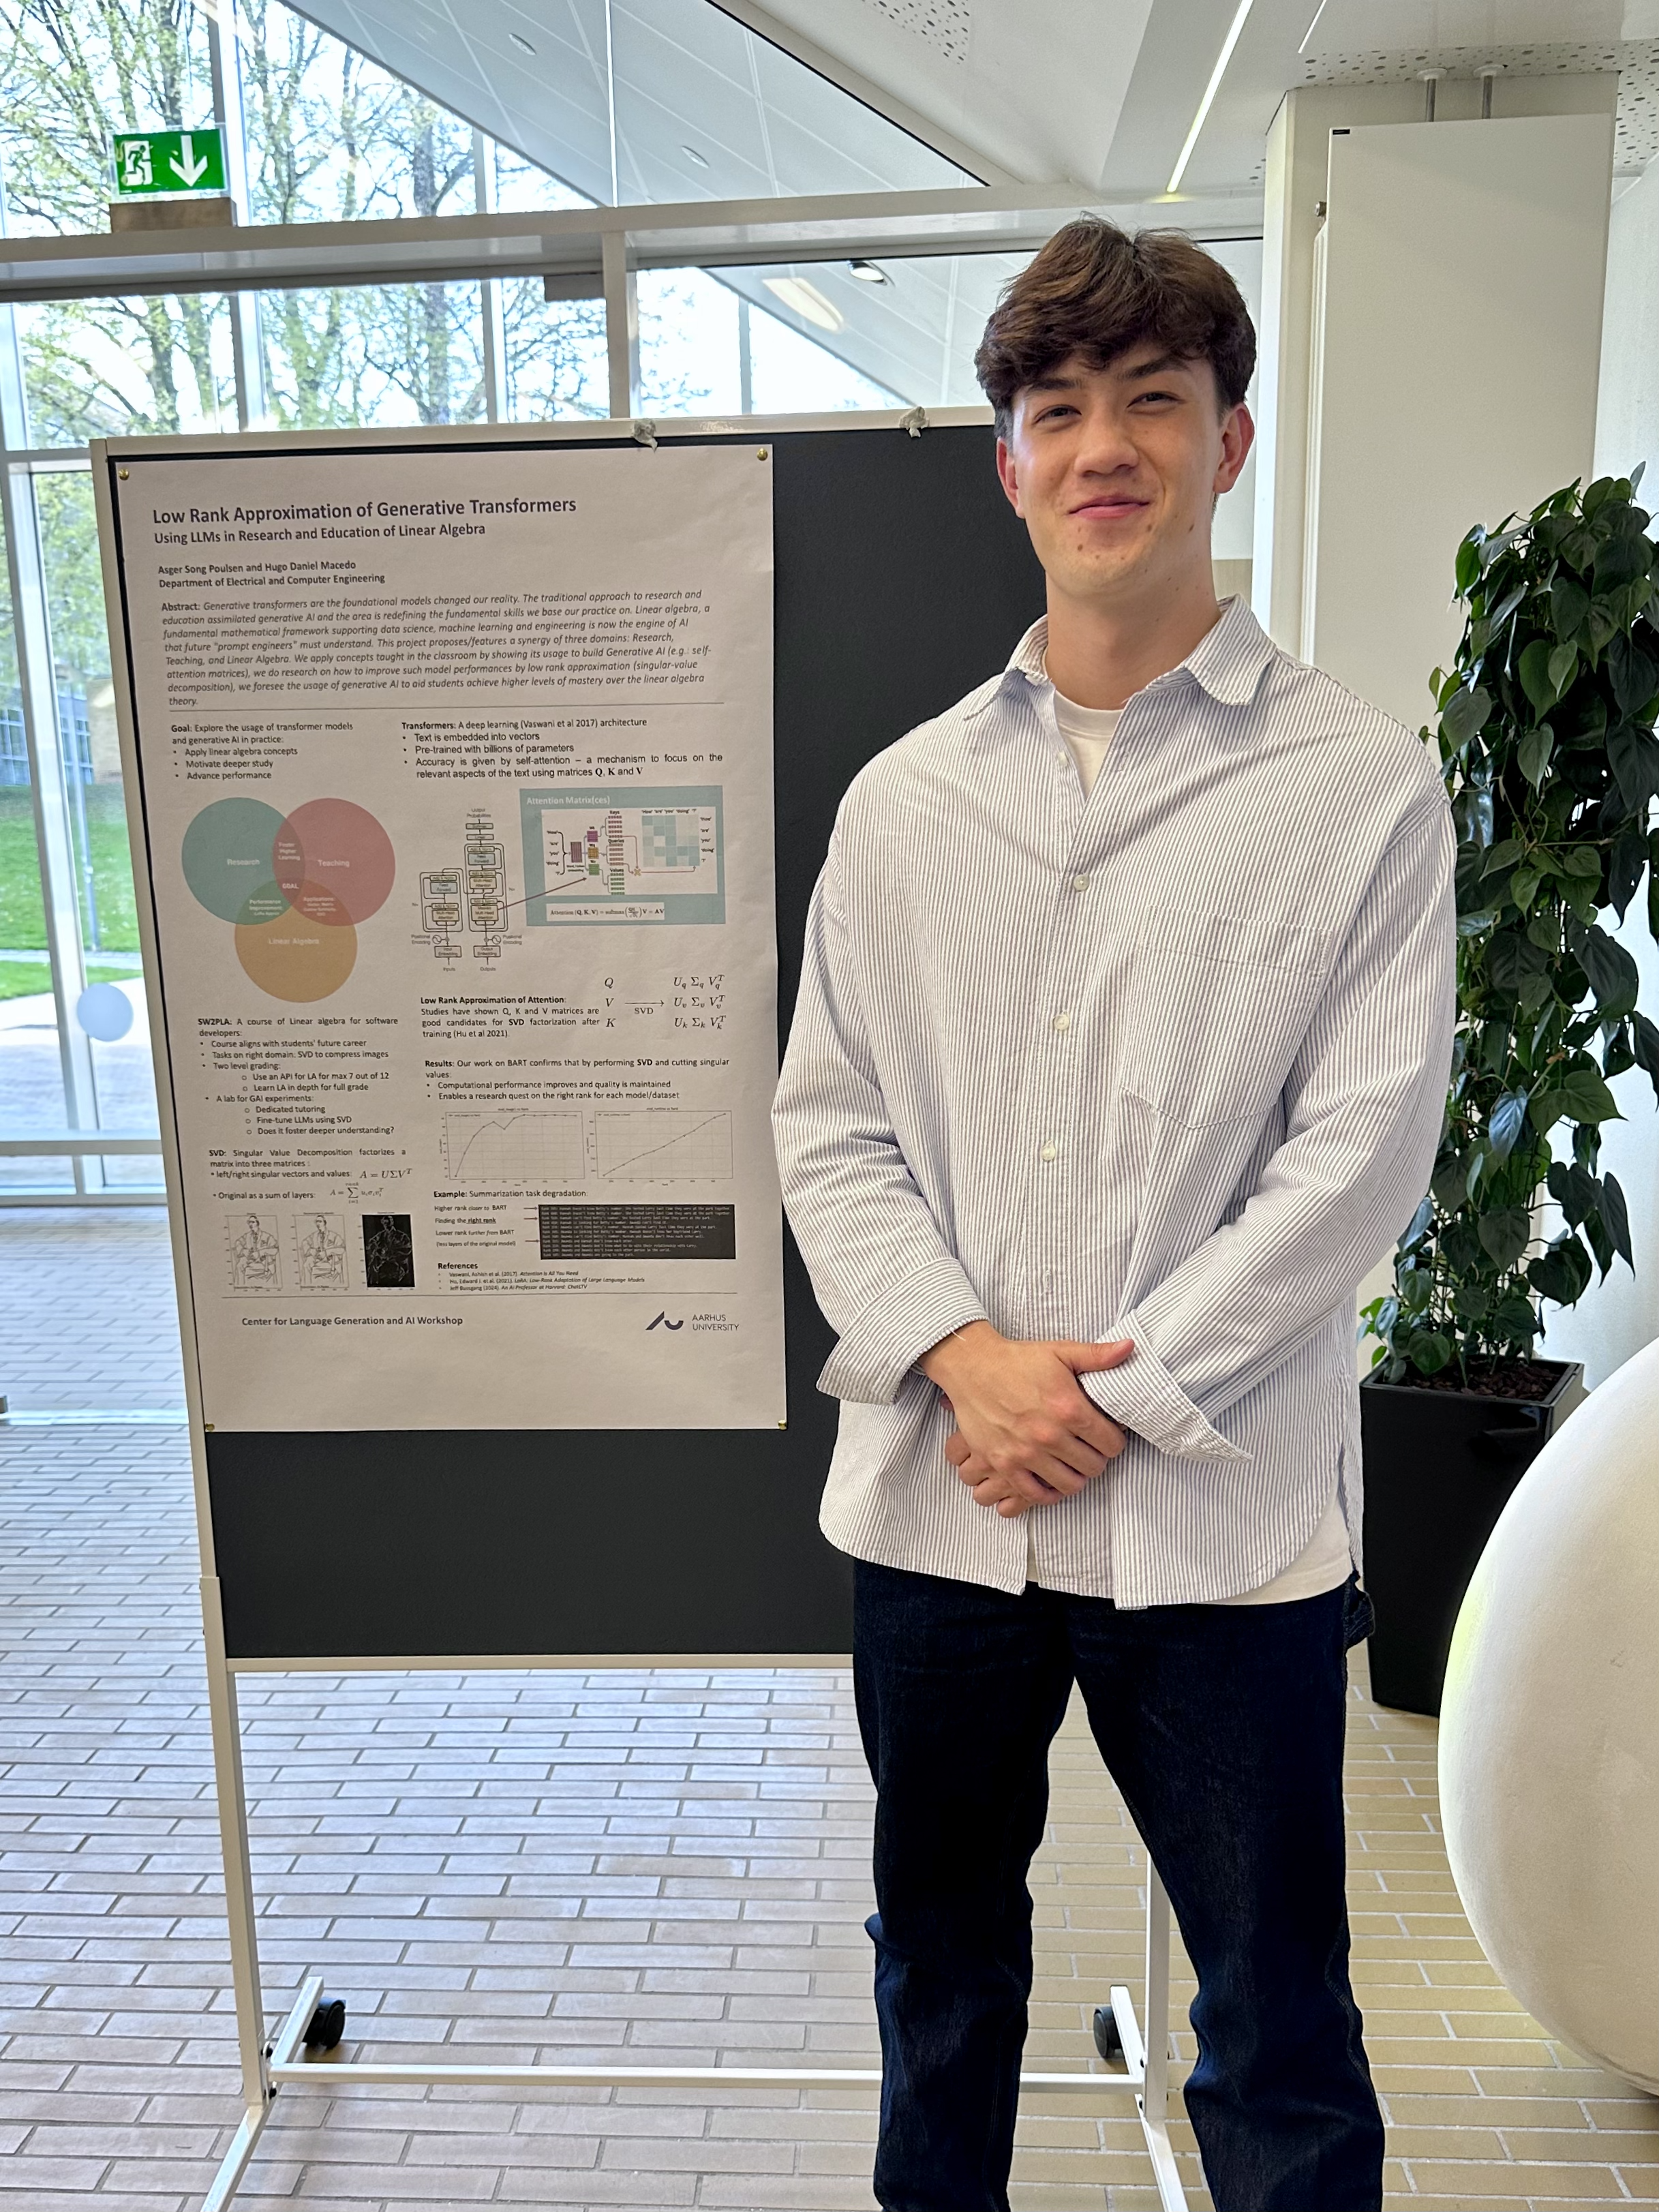
\includegraphics[width=0.6\textwidth]{figs/IMG_5113.png}
    \caption{3rd place in the CLAI Poster Competition}
    \label{fig:CLAI_Poster_Competition}
\end{figure}
It was an honor to represent the Department of Electrical and Computer Engineering (ECE) at such a forum. This accolade not only represents a personal achievement but also served as valuable practice for presenting research findings to a broader audience, including students and faculty members from various disciplines.

\section*{Conclusion}

The involvement in the SW2PLA course as a TA, while simultaneously conducting research for the bachelor's thesis, created a rich educational synergy. This experience not only enhanced the understanding and teaching of linear algebra but also allowed for the direct application and evaluation of theoretical concepts in practical, research-based applications. It underscores the importance of an integrated approach in education, where teaching responsibilities and academic research complement and enrich each other, preparing students for future challenges in technology and engineering.

\chapter{Interviews with CLAI Members}\label{appendix:Bergenholtz}
The Center for Language Generation and AI (CLAI) at Aarhus University is dedicated to researching and developing foundational language models. CLAI explores the implications of these models for understanding language and cognition, and addresses the ethical issues inherent in language generation and AI. Additionally, the center investigates the creative and pedagogical potential of these technologies. CLAI is a cross-disciplinary research program that integrates linguistics, humanities computing, cognitive science, media studies, and aesthetics.

As preparation for this bachelor's thesis, interviews were conducted with members of CLAI to gain insights into the current research and application of LLMs within the university. Furtherly, inspiration was sought for the development of a chatbot, specifally the issues and challenges that arise when implementing such a system in an academic setting.
Interviews were conducted with the following members of CLAI:

\section*{Customized RAG Chatbot at Aarhus University}
    Associate professor Carsten Bergenholtz from the Department of Management implemented, in collaboration with associate professor Oana Vuculescu, a RAG chatbot for his Philosophy of Science course at Aarhus University. For inspiration and guidance on the development of a RAG chatbot an informal interview was conducted with professor Bergenholtz. His involvement provided crucial insights that shaped the direction of the implementation of the chatbot related to this thesis.

    \subsection*{Interview Summary}

    During our discussions, concerns were raised about the use of chatbots like ChatGPT-4 in educational environments. While these systems can produce impressive outputs, they also pose risks due to potential inaccuracies and a lack of course-specific knowledge. However, solutions exist to mitigate these challenges. Professor Bergenholtz shared his experience with implementing a customized RAG chatbot for his Philosophy of Science course, which had an enrollment of 550 students.

    \subsection*{Chatbot Implementation}

    The customized chatbot was used approximately 20,000 times by the students, indicating strong engagement and utility. Professor Bergenholtz uploaded about 250 pages of course-relevant documents, from text to subtitles from his online lectures, to create a knowledge base for the chatbot. This setup, based on AU's Microsoft Azure platform, ensured that the chatbot was:

    \begin{itemize}
        \item GDPR compliant, adhering to data protection regulations.
        \item Based on the ChatGPT-4 model, ensuring advanced conversational capabilities.
        \item Freely accessible to all students, removing financial barriers.
        \item Equipped with an appealing user interface, enhancing user experience.
        \item Integrated within the existing university systems, ensuring seamless access.
    \end{itemize}
    \begin{figure}[H]
        \centering
        \includegraphics[width=0.6\textwidth]{figs/appcomponents.png}
        \caption{RAG patterns that include Azure AI Search from which Bergenholtz' chatbot was inspired from - taken from \cite{microsoft}}
        \label{fig:CLAI_Poster_Competition}
    \end{figure}

    The RAG chatbot was specifically designed to respond only to queries related to the course content. Questions outside the course scope received a 'cannot answer this' response to maintain the focus and academic integrity of the tool. Additionally, the chatbot provided a link to the source of its answers, enhancing transparency and trust.

    \subsection*{Chatbot Evaluation and Costs}

    The quality of the chatbot's responses was satisfactory, with about 85\% of interactions leading to useful answers, and only 2-4.5\% of responses being flawed. Notably, the flawed responses were quickly identified by users through follow-up questions. Despite its imperfections, the chatbot was considered a significant improvement over traditional search methods or regular chatbots used by students. The total cost of the chatbot was approximately 600€, with actual running costs around 400€ for 20,000 interactions, showcasing its cost-effectiveness.

    \subsection*{Student Feedback and Future Prospects}

    The chatbot was well-received based on survey responses, with students appreciating its ability to clarify complex concepts, compare texts, and summarize content. This tool proved particularly useful for large classes and when copyright for the necessary materials was held by the course instructor. Plans are in place to continue and enhance this service in future courses, focusing on guiding students to ask more effective questions.

    \subsection*{Conclusion}

    The implementation of the RAG chatbot at Aarhus University exemplifies the practical application of LLMs in enhancing educational experiences. The project set a precedent for future educational tools that leverage AI to support learning and inquiry. This initiative highlights the synergy between innovative technology and traditional educational practices, paving the way for more dynamic and interactive learning environments.

\section*{Introduction to Various Tools and Platforms for Development and Research of LLMs}
    Research assistant Rasmus Hansen from the Centre for Educational Development at Aarhus University specialises in research on students and teachers' practice with learning technology. His current focus is specifically on Generative AI, writing, and feedback. The interview with Rasmus provided valuable insights into some tools and platforms that can be used for developing and researching LLMs.
    \subsection*{Interview Summary}
        After presenting the goal of the thesis and the planned implementation of the chatbot, Rasmus provided an overview of the tools and platforms that could be beneficial for the project. The following tools/platforms were recommended:
        \begin{itemize}
            \item \textbf{Hugging Face:} A platform that provides access to pre-trained models, datasets, and training pipelines for NLP tasks.
            \item \textbf{GPT4ALL:} A free-to-use, locally running, privacy-aware chatbot where no GPU or internet is required. Furtherly, a guide on how use RAG in GPT4ALL was provided.\footnote{\url{https://docs.gpt4all.io/gpt4all_chat.html}}
            \item \textbf{LMStudio:} A platform that allows users to create, train, and deploy custom language models locally.
        \end{itemize}
        As the project progressed only the Hugging Face platform was used for this thesis. The platform provided access to the pre-trained BART model, and allowed for fine-tuning on custom datasets. The introduction to Hugging Face was instrumental in easy access to the BART model and the implementation of the case study: Low Rank Approximation.
\chapter{Architecture of BART}
    \label{appendix:BART}
    One can inspect the model architecture by using the \texttt{transformers} library by Hugging Face.
    \section*{BART-Base}
    \begin{listing}[H]
        \begin{minted}{python}
from transformers import AutoModelForSeq2SeqLM
model_checkpoint = "facebook/bart-base"
model = AutoModelForSeq2SeqLM.from_pretrained(model_checkpoint)
        \end{minted}
        \caption{Loading pre-trained BART-base model from the Hugging Face model repository}
        \label{lst:bart_base_fetch}
    \end{listing}
    This code snippet fetches the configuration, tokenizer, and weights of the BART model from the Hugging Face model repository. The model can be inspected by printing the model object, which will output the model architecture as shown in Listing \ref{lst:bart_base_architecture}.
    \newpage
    \begin{listing}[H]
                \begin{minted}[fontsize=\footnotesize]{python}
BartForConditionalGeneration(
  (model): BartModel(
    (shared): Embedding(50265, 768, padding_idx=1)
    (encoder): BartEncoder(
      (embed_tokens): BartScaledWordEmbedding(50265, 768, padding_idx=1)
      (embed_positions): BartLearnedPositionalEmbedding(1026, 768)
      (layers): ModuleList(
        (0-5): 6 x BartEncoderLayer(
          (self_attn): BartSdpaAttention(
            (k_proj): Linear(in_features=768, out_features=768, bias=True)
            (v_proj): Linear(in_features=768, out_features=768, bias=True)
            (q_proj): Linear(in_features=768, out_features=768, bias=True)
            (out_proj): Linear(in_features=768, out_features=768, bias=True)
          )
          (self_attn_layer_norm): LayerNorm((768,), eps=1e-05, elementwise_affine=True)
          (activation_fn): GELUActivation()
          (fc1): Linear(in_features=768, out_features=3072, bias=True)
          (fc2): Linear(in_features=3072, out_features=768, bias=True)
          (final_layer_norm): LayerNorm((768,), eps=1e-05, elementwise_affine=True)
        )
      )
      (layernorm_embedding): LayerNorm((768,), eps=1e-05, elementwise_affine=True)
    )
    (decoder): BartDecoder(
      (embed_tokens): BartScaledWordEmbedding(50265, 768, padding_idx=1)
      (embed_positions): BartLearnedPositionalEmbedding(1026, 768)
      (layers): ModuleList(
        (0-5): 6 x BartDecoderLayer(
          (self_attn): BartSdpaAttention(
            (k_proj): Linear(in_features=768, out_features=768, bias=True)
            (v_proj): Linear(in_features=768, out_features=768, bias=True)
            (q_proj): Linear(in_features=768, out_features=768, bias=True)
            (out_proj): Linear(in_features=768, out_features=768, bias=True)
          )
          (activation_fn): GELUActivation()
          (self_attn_layer_norm): LayerNorm((768,), eps=1e-05, elementwise_affine=True)
          (encoder_attn): BartSdpaAttention(
            (k_proj): Linear(in_features=768, out_features=768, bias=True)
            (v_proj): Linear(in_features=768, out_features=768, bias=True)
            (q_proj): Linear(in_features=768, out_features=768, bias=True)
            (out_proj): Linear(in_features=768, out_features=768, bias=True)
          )
          (encoder_attn_layer_norm): LayerNorm((768,), eps=1e-05, elementwise_affine=True)
          (fc1): Linear(in_features=768, out_features=3072, bias=True)
          (fc2): Linear(in_features=3072, out_features=768, bias=True)
          (final_layer_norm): LayerNorm((768,), eps=1e-05, elementwise_affine=True)
        )
      )
      (layernorm_embedding): LayerNorm((768,), eps=1e-05, elementwise_affine=True)
    )
  )
  (lm_head): Linear(in_features=768, out_features=50265, bias=False)
)
                \end{minted}
                \caption{BART-base model architecture}
                \label{lst:bart_base_architecture}
            \end{listing}
The model has a total of \(139\) million parameters.

\section*{BART-Large}
Similarly, for the BART-large model:
\begin{listing}[H]
    \begin{minted}{python}
from transformers import AutoModelForSeq2SeqLM
model_checkpoint = "facebook/bart-large"
model = AutoModelForSeq2SeqLM.from_pretrained(model_checkpoint)
    \end{minted}
    \caption{Loading pre-trained BART-large model from the Hugging Face model repository}
    \label{lst:bart_large_fetch}
\end{listing}
    The model architecture is shown in Listing \ref{lst:bart_large_architecture}.
        \begin{listing}[H]
                \begin{minted}[fontsize=\footnotesize]{python}
BartForConditionalGeneration(
  (model): BartModel(
    (shared): Embedding(50265, 1024, padding_idx=1)
    (encoder): BartEncoder(
      (embed_tokens): BartScaledWordEmbedding(50265, 1024, padding_idx=1)
      (embed_positions): BartLearnedPositionalEmbedding(1026, 1024)
      (layers): ModuleList(
        (0-11): 12 x BartEncoderLayer(
          (self_attn): BartSdpaAttention(
            (k_proj): Linear(in_features=1024, out_features=1024, bias=True)
            (v_proj): Linear(in_features=1024, out_features=1024, bias=True)
            (q_proj): Linear(in_features=1024, out_features=1024, bias=True)
            (out_proj): Linear(in_features=1024, out_features=1024, bias=True)
          )
          (self_attn_layer_norm): LayerNorm((1024,), eps=1e-05, elementwise_affine=True)
          (activation_fn): GELUActivation()
          (fc1): Linear(in_features=1024, out_features=4096, bias=True)
          (fc2): Linear(in_features=4096, out_features=1024, bias=True)
          (final_layer_norm): LayerNorm((1024,), eps=1e-05, elementwise_affine=True)
        )
      )
      (layernorm_embedding): LayerNorm((1024,), eps=1e-05, elementwise_affine=True)
    )
    (decoder): BartDecoder(
      (embed_tokens): BartScaledWordEmbedding(50265, 1024, padding_idx=1)
      (embed_positions): BartLearnedPositionalEmbedding(1026, 1024)
      (layers): ModuleList(
        (0-11): 12 x BartDecoderLayer(
          (self_attn): BartSdpaAttention(
            (k_proj): Linear(in_features=1024, out_features=1024, bias=True)
            (v_proj): Linear(in_features=1024, out_features=1024, bias=True)
            (q_proj): Linear(in_features=1024, out_features=1024, bias=True)
            (out_proj): Linear(in_features=1024, out_features=1024, bias=True)
          )
          (activation_fn): GELUActivation()
          (self_attn_layer_norm): LayerNorm((1024,), eps=1e-05, elementwise_affine=True)
          (encoder_attn): BartSdpaAttention(
            (k_proj): Linear(in_features=1024, out_features=1024, bias=True)
            (v_proj): Linear(in_features=1024, out_features=1024, bias=True)
            (q_proj): Linear(in_features=1024, out_features=1024, bias=True)
            (out_proj): Linear(in_features=1024, out_features=1024, bias=True)
          )
          (encoder_attn_layer_norm): LayerNorm((1024,), eps=1e-05, elementwise_affine=True)
          (fc1): Linear(in_features=1024, out_features=4096, bias=True)
          (fc2): Linear(in_features=4096, out_features=1024, bias=True)
          (final_layer_norm): LayerNorm((1024,), eps=1e-05, elementwise_affine=True)
        )
      )
      (layernorm_embedding): LayerNorm((1024,), eps=1e-05, elementwise_affine=True)
    )
  )
  (lm_head): Linear(in_features=1024, out_features=50265, bias=False)
)
                \end{minted}
                \caption{BART-large model architecture}
                \label{lst:bart_large_architecture}
            \end{listing}
    The model has a total of \(406\) million parameters.

\end{document}
